\begin{usecase}{View Integrated Calendar}
  \ucbasicinfo{High}{Regular}
  \ucshortdescription{Allows users to view their integrated calendar}
  \uctrigger{User selects the option to view the integrated calendar.}
  \ucactors{User}{None}
  \ucpreconditions{User must be logged into the system.}
  \ucrelationships{N/A}{N/A}{N/A}
  \ucinputsoutputs{
    \begin{itemize}
      \item \textbf{Integrated calendar} (Source: System)
    \end{itemize}
  }{
    \begin{itemize}
      \item \textbf{Integrated calendar} (Destination: App)
    \end{itemize}
  }
  \ucmainflow{
    \begin{enumerate}
      \item The user clicks on the integrated calendar.
            \ucinfo{The system displays the all integrated calendars and it's events}
    \end{enumerate}
  }
  \ucconclusion{User successfully views their integrated calendar with all the events.}
  \ucpostconditions{The integrated calendar is displayed}
  \ucspecialrequirements{N/A}
  \ucbusinessrules{
    \begin{itemize}
      \item \textbf{Events must be displayed according to user preferences .}
    \end{itemize}
  }
\end{usecase}

\begin{figure}[!h]
  \centering
  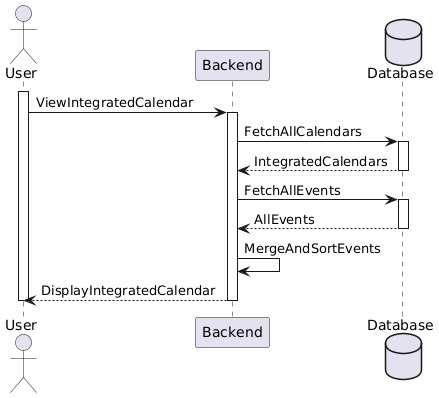
\includegraphics[width=\textwidth]{images/docs/diagrams/sequence-diagrams/all-sequence-diagrams/View Integrated Calendar.png}
  \caption{View Integrated Calendar Sequence Diagram}
  \label{fig:seq/view-integrated-calendar}
\end{figure}